\documentclass{article}
\usepackage[utf8]{vntex}
\usepackage{amsmath}
\usepackage{amsopn}
\usepackage{tikz}
\usetikzlibrary{matrix}

\title{Linear Algebra}
\author{Vinh Vũ}
\date{11.17.2025}

\begin{document}
\section{Matrics - Ma Trận}
\subsection{Determinant - Định Thức}

\subsubsection{Hoán Vị}
Cho ma trận
$A = \begin{pmatrix}
  1 & 2 & 3\\
  4 & 5 & 6\\
  7 & 8 & 9
\end{pmatrix}$
. Hoán vị ma trận A tức là sắp xếp các phần tử của ma trận A theo thức tự khác nhau.
$$
\begin{pmatrix}
  1 & 2 & 3\\
  4 & 5 & 6\\
  7 & 8 & 9
\end{pmatrix}\rightarrow
\begin{pmatrix}
  2 & 3 & 1\\
  7 & 9 & 8\\
  6 & 5 & 4
\end{pmatrix}
$$

\subsubsection{Nghịch Thế}
Là số cặp hai chữ số mà ở đó số trước lớn hơn số sau. Ký hiệu là N.
\\Từ dãy số$A=\{3,4,5,2,1\}$. Ta có các cặp số nghịch thế sau:
\\(3,2); (3,1); (4,2); (4,2); (5,2); (5,2); (2,1)
\\$\Rightarrow N = 7$

\subsubsection{Ma Trận Vuông Cấp n}
Giả sử ma trận A là ma trận vuông cấp 2.
$$
|A| = 
\begin{vmatrix}
  a & b \\
  c & d
\end{vmatrix} = a*d - b*c
$$
Giả sử ma trận B là ma trận vuông cấp 3
$$
|B| = 
\begin{vmatrix}
  a & b & c\\
  d & e & f\\
  g & h & i
\end{vmatrix}
$$
Theo công thức đồ thị sau:
$$ 
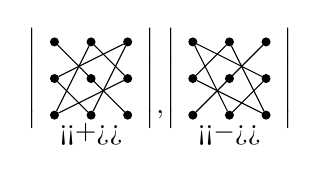
\begin{tikzpicture}
\matrix[matrix of nodes,left delimiter=|,right delimiter=|,
  row sep=1em,column sep=1em,
  nodes={draw,fill,circle,inner sep=1pt},nodes in empty cells] (m) at (0,0) {
    & & \\
    & & \\
    & & \\
  };
  \draw (m-2-1) -- (m-3-2);
  \draw (m-1-1) -- (m-3-3);
  \draw (m-1-2) -- (m-2-3);
  %
  \draw (m-1-2) -- (m-3-1);
  \draw (m-1-3) -- (m-3-2);
  %
  \draw (m-2-1) -- (m-1-3);
  \draw (m-3-1) -- (m-2-3);

  \matrix[matrix of nodes,left delimiter=|,right delimiter=|,
  row sep=1em,column sep=1em,
  nodes={draw,fill,circle,inner sep=1pt},nodes in empty cells] (n) at (5em,0) {
    & & \\
    & & \\
    & & \\
  };
  \draw (n-2-3) -- (n-3-2);
  \draw (n-1-3) -- (n-3-1);
  \draw (n-1-2) -- (n-2-1);
  %
  \draw (n-1-2) -- (n-3-3);
  \draw (n-1-1) -- (n-3-2);
  %
  \draw (n-2-3) -- (n-1-1);
  \draw (n-3-3) -- (n-2-1);

  \node at (0.0em,-2em) {<<$+$>>};
  \node at (2.5em,0 |- m.base) {$,$};
  \node at (5.0em,-2em) {<<$-$>>};
\end{tikzpicture}
$$
Ta có $|B| = aei + bfg + cdh - ceg - bdi - afh$
\\Có thể bấm máy tính để tính nhanh với những ma trận có cấp $n\geq4$.
\subsubsection{Định Thức Con}
\subsubsection{Phần Bù Đại Số}
\subsubsection{Tính Chất Định Thức}
\subsubsection{Biến Đổi Sơ Cấp}

\end{document}